
\documentclass[a4paper,UKenglish,cleveref, autoref]{socg-lipics-v2019}
%This is a template for producing LIPIcs articles. 
%See lipics-manual.pdf for further information.
%for A4 paper format use option "a4paper", for US-letter use option "letterpaper"
%for british hyphenation rules use option "UKenglish", for american hyphenation rules use option "USenglish"
%for section-numbered lemmas etc., use "numberwithinsect"
%for enabling cleveref support, use "cleveref"
%for enabling cleveref support, use "autoref"
%\graphicspath{{./graphics/}}%helpful if your graphic files are in another directory

\bibliographystyle{plainurl}% the mandatory bibstyle
\graphicspath{{images/}}
\DeclareGraphicsExtensions{.pdf,.png,.jpg}
\lstset{
	language=Java,
	breaklines,
}

\title{Unified data structures for solving optimally a set of interrelated computational geometry problems} 
\titlerunning{Data structures for solving a set of computational geometry problems}%optional, please use if title is longer than one line

\author{Vasyl Tereshchenko}{
	Faculty of computer science and cybernetics, Taras Shevchenko National University of Kyiv, Ukraine}
{vtereshch@gmail.com}{}{}%TODO mandatory, please use full name; only 1 author per \author macro; first two parameters are mandatory, other parameters can be empty. Please provide at least the name of the affiliation and the country. The full address is optional
%\footnote{}
\author{Semen Chudakov}{Faculty of computer science and cybernetics, Taras Shevchenko National University of Kyiv, Ukraine}
{semen.chudakov7@gmail.com}{}{}

\authorrunning{V. Tereshchenko and S. Chudakov}%TODO mandatory. First: Use abbreviated first/middle names. Second (only in severe cases): Use first author plus 'et al.'

\Copyright{Vasyl Tereshchenko and Semen Chudakov}%TODO mandatory, please use full first names. LIPIcs license is "CC-BY";  http://creativecommons.org/licenses/by/3.0/

\ccsdesc[500]{Theory of computation~Computational geometry}%TODO mandatory: Please choose ACM 2012 classifications from https://dl.acm.org/ccs/ccs_flat.cfm 

\keywords{Algorithmic tools,   Computational geometry, Interrelated problems set, Unified algorithmic environment, Concatenable queue}%TODO mandatory; please add comma-separated list of keywords

\category{}%optional, e.g. invited paper

\relatedversion{}%optional, e.g. full version hosted on arXiv, HAL, or other respository/website
%\relatedversion{A full version of the paper is available at \url{...}.}

\supplement{}%optional, e.g. related research data, source code, ... hosted on a repository like zenodo, figshare, GitHub, ...

%\funding{(Optional) general funding statement \dots}%optional, to capture a funding statement, which applies to all authors. Please enter author specific funding statements as fifth argument of the \author macro.

\acknowledgements{}%optional

%\nolinenumbers %uncomment to disable line numbering

%\hideLIPIcs  %uncomment to remove references to LIPIcs series (logo, DOI, ...), e.g. when preparing a pre-final version to be uploaded to arXiv or another public repository

%Editor-only macros:: begin (do not touch as author)%%%%%%%%%%%%%%%%%%%%%%%%%%%%%%%%%%
\EventEditors{}
\EventNoEds{2}
\EventLongTitle{36th International Symposium on Computational Geometry (SoCG 2020)}
\EventShortTitle{SoCG 2020}
\EventAcronym{SoCG}
\EventYear{2020}
\EventDate{June  23--26, 2020}
\EventLocation{Zürich, Switzerland}
\EventLogo{socg-logo}
\SeriesVolume{}
\ArticleNo{}
%%%%%%%%%%%%%%%%%%%%%%%%%%%%%%%%%%%%%%%%%%%%%%%%%%%%%%

\begin{document}

\maketitle

%TODO mandatory: add short abstract of the document
\begin{abstract}
	The paper is devoted to the development and  of an efficient algorithmic model for solving a set of interrelated computational geometry problems. To do this, a unified algorithmic environment with unified data structures is created, which allows to implement complex use cases efficiently with respect to computational resources. We build the environment on the basis of the ``divide and conquer'' strategy. 
	Once a convex hull is key to a set of computational geometry problems, we offer a concatenable queue data structure to maintain it. The data structure is implemented in a form of a binary tree. This allows to perform operations needed in algorithm for a set of problems in $O(\log n)$ time. Furthermore we offer a way to execute the algorithms both sequentially and in parallel.
	In the future the algorithmic environment can be improved to support other computational models with similar properties for solving problems. As an example, the Voronoi diagram or the Delaunay triangulation can be considered.
\end{abstract}

\section{Introduction}
\label{sec:introduction}

	Nowadays, advanced computer simulations and visualizing of complex scientific researches as well as large scale technical projects requires to simultaneously solve a set of problems. The core of this set are problems of computational geometry and computer graphics. To solve such problems it is needed to create suitable algorithmic frameworks, that would yield accurate results in real time. Existing methods (iLastic \cite{ilastik}, IMARIS \cite{imaris}, ImageJ \cite{imagej}), that are based on a set of algorithms implementations organized in a package does not result in desirable efficiency and accuracy. It is worth noting, that there are a lot of parallel algorithms designed to solve specifically certain computational geometry problems such as in \cite{aggarwal,atallah,cole,amato,chen,berkman,goodman,akl,jaja,leeuwen,reif}. Every such algorithm requires its own computational resources and is executed independently from others. In such case some identical steps, such as preprocessing and building data structures, are performed several times. 
	
	Therefore, an important objective in developing the algorithmic models is to create a universal tool, which would have means to efficiently solve a set of problems. This tool should also execute identical steps of the algorithms once and be able to represent results of those steps in a form of the unified data structures. In \cite{tereshchenko} the notion of a unified algorithmic environment is introduced, which is based on the ``divide-and-conquer'' principle and takes into account the aforementioned features of the algorithms. In particular, the preprocessing and splitting the initial set of data to form the recursion tree is common for all problems and is executed only once. During the merge stage intermediate results are maintained in a weighted concatenable queue. This model does not repeat computations and the intermediate results are highly reused during the algorithms, which yields good performance.
	
	In this article we first describe how the convex hull algorithm for a static set of points is decomposed into separate stages and incorporated into our unified algorithmic environment model (UAEM). Then we provide detailed explanation on how the concatenable queue which is used in the algorithm is implemented. Finally we make complexity analysis for the algorithm and evaluate its performance.


\section{Unified algorithmic environment}
\label{sec:unified-algorithmic-environment}
\subsection{Algorithms stages}


% //////////////////////////////////////////////////////////////////////////////////////////////////////////////////////////
% ----------------------------------------------- PROBLEM STATEMENT --------------------------------------------------------
% //////////////////////////////////////////////////////////////////////////////////////////////////////////////////////////
	
	
	In this section we describe the principle of how we decompose each algorithm into distinct parts. This partition is then used to avoid repeating the computations in the algorithmic environment. The principle will be show on a convex hull algorithm which is similar to the one describe in \cite{overmars} but operates on a static set of points.
	
	The notion of a convex hull is simple. For a set of points $S$ in a $k$-dimensional space it is a smallest convex set, that comprise $S$. In practice to solve such problem, means to find a subset in $S$, which can be a "skeleton" for the convex hull.
	
	
% //////////////////////////////////////////////////////////////////////////////////////////////////////////////////////////
% ----------------------------------------------- PREPROCESSING ------------------------------------------------------------
% //////////////////////////////////////////////////////////////////////////////////////////////////////////////////////////
	
	
	In the preprocessing stage, the "inner" points, which lie on a horizontal or vertical line, are removed from the set. Formally, the removal criterion is formulated as follows. For $a = (x_a, y_a)$ we denote $x(a)=x_a$, $y(a)=y_a$. Let points $a_1, a_2, ..., a_k$ lie on one horizontal line and $x(a_1) < x(a_2) <... <x (a_k) $. Then, by the criterion, the points $a_2, a_3, ..., a_{k-1}$ must be removed. Analogously for the vertical case.
	
	Consider an algorithm that, in a sorted array, for each group of identical elements, deletes all but the first and the last one (if there are more than two repetitions). The idea behind the algorithm is to use two pointers technique to delete repetitions by overwriting their place with other non-repeating element. This way, additional memory usage can be reduced to a constant value. The algorithm makes one pass through the array. At each step, a constant amount of work is performed to decide whether to delete the current item. Given this, the complexity of the above algorithm is $O(n)$.
	
	To perform the preprocessing described above, it is needed to:
	
	\begin{enumerate}
		\item
		Sort points by $y$ (if $y$ coordinates are equal, the $x$ coordinates are compared).
		\item
		Delete repetitions by $y$ coordinate using the described algorithm.
		\item
		Sort points by $x$ (if $x$ coordinates are equal, the $y$ coordinates are compared).
		\item
		Delete repetitions by $x$ coordinate using the described algorithm.
	\end{enumerate}
	
	In the result we get a set of points for which we can apply the recursive convex hull algorithm.
	
	% //////////////////////////////////////////////////////////////////////////////////////////////////////////////////////////
	% ----------------------------------------------- SPLIT ------------------------------------------------------------
	% //////////////////////////////////////////////////////////////////////////////////////////////////////////////////////////
	
	
	At the stage of splitting the initial problem, the set of points is divided into left and right parts of equal size. Since a array-like data structure is used to store the points, this operations can be completed in $O(1)$ using the formula below:
	
	\begin{equation}
		M_{i,j}=\frac{i+j}{2}
	\end{equation}
	The recursion stops when there are no more than $3$ points in the set.
	
	For the base case, the set of points can have $2$ or $3$ elements. In the first case the highest of two points forms the upper part of the hull, and the lower - the lower part. To consider the base case of $3$ points, we introduce an additional notion of the tangent slope given by two points on the plane. For arbitrary points $a_1, a_2$ such that $x(a_1)<x(a_2)$ slope is denoted as $\lambda$:
	
	\begin{equation}
	\lambda(a_1, a_2)=\frac{y(a_2)-y(a_1)}{x(a_2)-x(a_1)}
	\end{equation}

% //////////////////////////////////////////////////////////////////////////////////////////////////////////////////////////
% --------------------------------   THE MERGE STEP ------------------------------------------------------------------------
% //////////////////////////////////////////////////////////////////////////////////////////////////////////////////////////

	
	In \cite{overmars} an algorithm for merging two convex hulls is described. The idea of this algorithm is to maintain the hull in two concatenated queues. The hull is divided into two parts. In this article it is divided into the upper and the lower sub-hulls. Then, using the two-pointer technique and the cases described in \cite{overmars}, the proper tangent line is searched. It remains to split the two queues at the found vertices that form the tangent and to merge the remaining parts. An example of performing such a procedure is shown in Fig. \ref{fig:ch_union}.
	
	\begin{figure}[t]
		\centering
		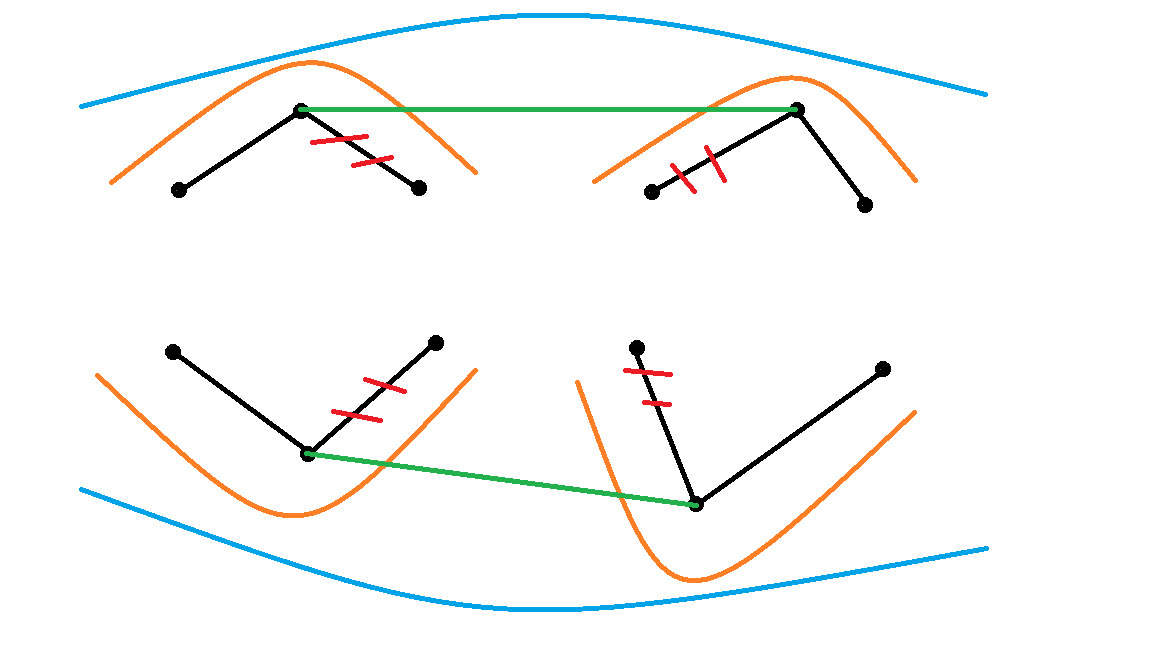
\includegraphics[width=0.8\textwidth, height=0.3\textheight]{ch_union}
		\caption{Merging step of two hulls}
		\label{fig:ch_union}
	\end{figure}
	
	It remains to consider the corner cases that arise when performing the merging. The first of these cases is related to the ambiguity of the position of the utmost points in the described representation. The leftmost point of the left hull and the rightmost point of the right hull must belong to the upper parts of the view before finding the tangent line, because otherwise such tangent may be found incorrectly. An example of such incorrect search is given in Fig. \ref{fig:incorect_search}.
	
	\begin{figure}[t]
		\centering
		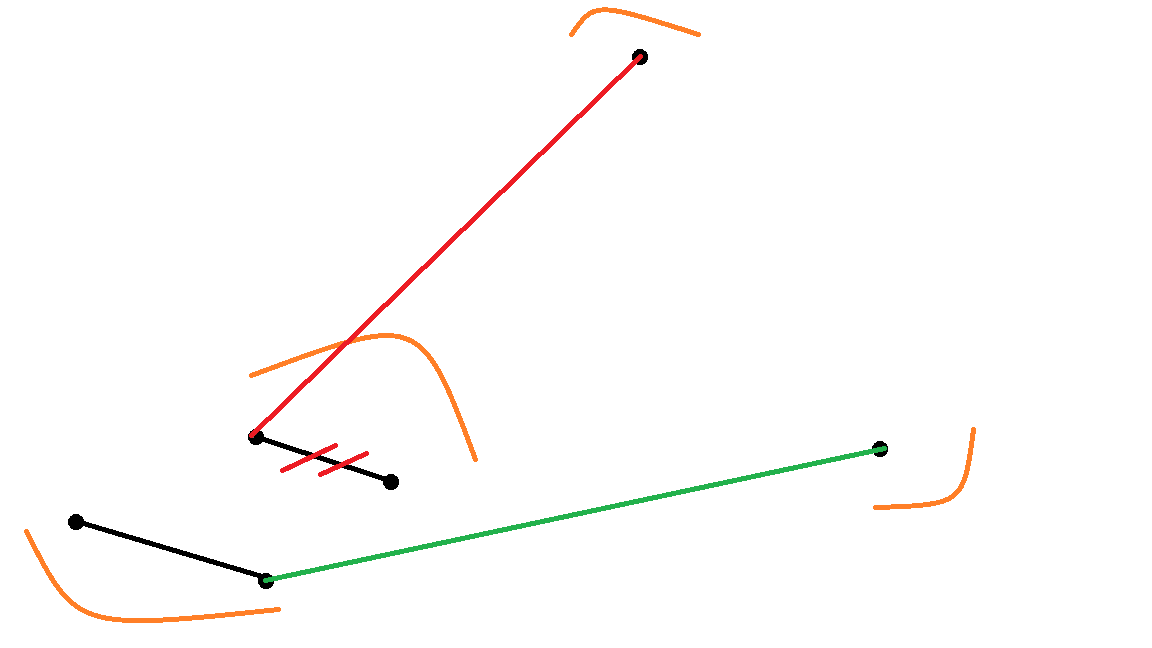
\includegraphics[width=0.8\textwidth, height=0.3\textheight]{incorect_search}
		\caption{Example of an incorrect position of the utmost left in the left sub-hull}
		\label{fig:incorect_search}
	\end{figure}
	
	To avoid such a situation, it is necessary to move the indicated points to the upper sub-hulls before merging them. For the rightmost point of the left hull and the leftmost point of the right hull we have the following cases. Similarly to the previous argument, they must be transferred to the upper parts of the hulls. And after merging these points must be transferred to the lower parts of the hull, if they do not belong to the resulting upper part of the final hull. Otherwise, the formed hull may be incorrect. An example of such case is shown in Fig. \ref{fig:incorect_edge_points}.
	
	
	\begin{figure}[t]
		\centering
		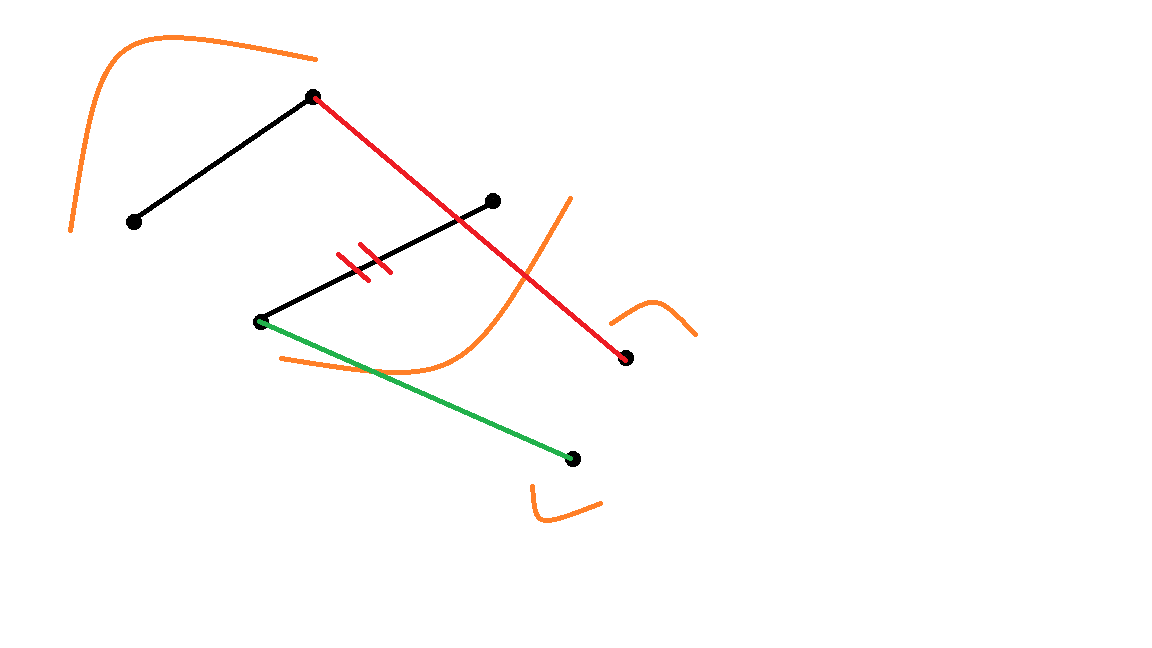
\includegraphics[width=0.8\textwidth, height=0.3\textheight]{incorect_edge_points}
		\caption{Example of a convex hull for a wrong position of the utmost left points of the left sub-hull}
		\label{fig:incorect_edge_points}
	\end{figure}
	
	After combining the parts of the convex hulls, another corner case might take place. The search for the tangent for the upper parts of the hulls does not take into account the position of the lower parts and vice versa. As a result, the upper and lower parts of the final hull may not form a coherent structure. An example of such a situation is shown in Fig. \ref{fig:incorect_lower_subhull}.
	
	\begin{figure}[t]
		\centering
		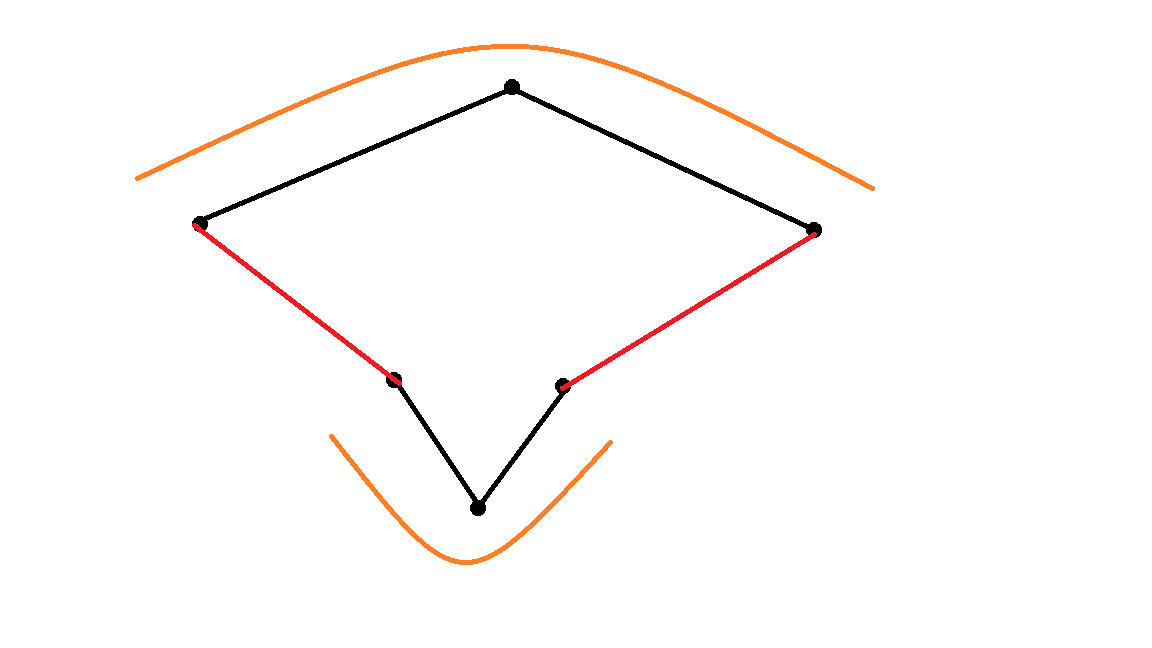
\includegraphics[width=0.8\textwidth, height=0.3\textheight]{incorect_lower_subhull}
		\caption{An example of a non-integral hull after merging along the reference lines}
		\label{fig:incorect_lower_subhull}
	\end{figure}
	
	To avoid such a situation, it is necessary to perform the step of cutting off the redundant parts of the formed lower sub-hull. Then searching for the left and right pivoting vertices in the concatenable queue is performed. After that, the queue is split over the found vertices. Fig. \ref{fig:correct_convex_hull} shows correct convex hull.
	
	\begin{figure}[t]
		\centering
		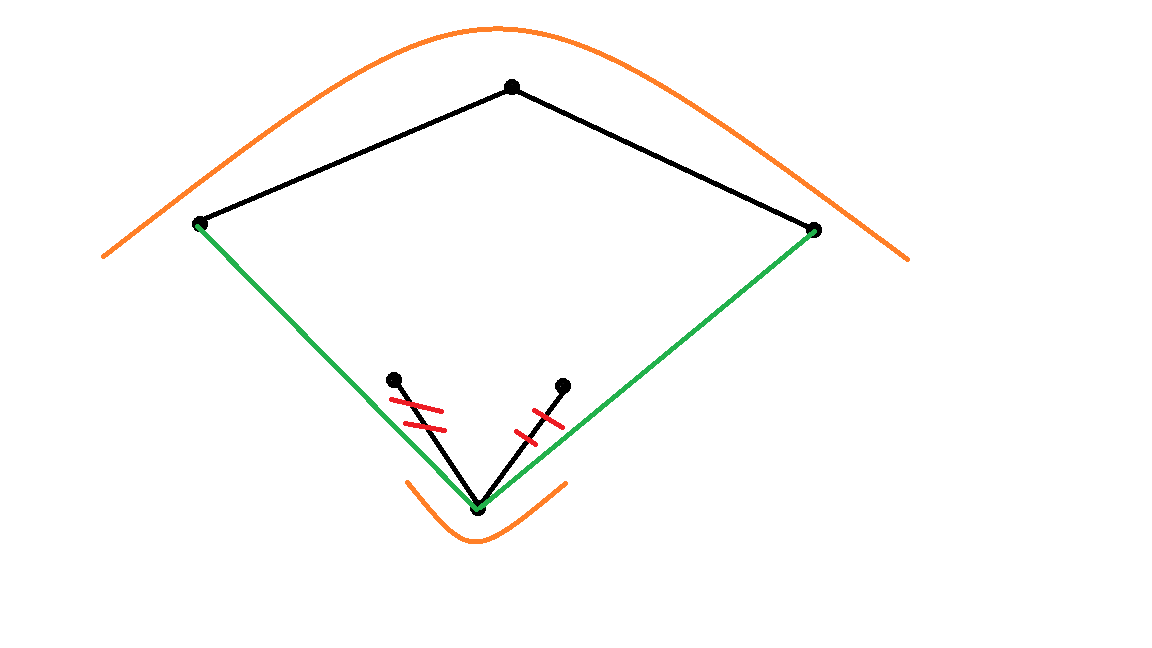
\includegraphics[width=0.8\textwidth, height=0.3\textheight]{correct_convex_hull}
		\caption{Correctly constructed convex hull}
		\label{fig:correct_convex_hull}
	\end{figure}



\subsection{``Divide-and-conquer'' algorithm interface}


	The next goal of this work is to build a unified algorithmic environment. The construction of such an object requires the combination of an algorithmic database together with the necessary data structures.  In fact, it is needed to create an interface of generic algorithm based on ``divide-and-conquer'' strategy, which will then be used on a specific input data.
	
	We start creating the generic interface by listing its components:
	
	\begin{itemize}
		\item 
		Preprocessing.
		\item 
		Splitting task into sub-tasks.
		\item 
		Solving sub-tasks.
		\item 
		Merging obtained results.
		\item 
		Checking, if a given input data is a base case for the algorithm.
		\item 
		Solving the base case.
	\end{itemize}
	
	Each of these components will represent a function in the future interface. Here there is a clear separation between the input type for the algorithm and the type of the result it returns. These two types should be parameters of the algorithm model. One should also pay attention to the input and output types of functions  in the interface.
	
	A large number of computational geometry algorithms, such as computing minimal spanning tree, the Delaunay triangulation, the Voronoi diagram and the convex hull accept the list of points. However, it would be wrong to limit the input type in the algorithm interface to a list of points. The reason for this is the fact that some algorithms can use the results of other algorithms as input data. A well known example is the construction of a Delaunay triangulation based on the Voronoi diagram maintained in a special data structure.
	
	Listing \ref{lst:algmodel} shows the constructed algorithm model. $IT$ denotes the input type and $OT$ - output type.
	
	\begin{lstlisting}[caption={Algorithm model based on the ``divide-and-conquer'' principle},label={lst:algmodel},captionpos=t,float,abovecaptionskip=-\medskipamount]
interface DaCAlgorithm[IT, OT]:
    boolean isBaseCase(IT input)
    int inputSize(IT input)

    OT solveBaseCase(IT input)
    IT preprocess(IT input)

    OT merge(OT first, OT second)
    Pair[IT, IT] divide(IT input)
	\end{lstlisting}
	
	
\section{Algorithm analysis and performance evaluation}
\label{sec:algorithm-analysis-and-performance-evaluation}
\subsection{Complexity}

% //////////////////////////////////////////////////////////////////////////////////////////////////////////////////////////
% ----------------------------------------------- COMPLEXITY ---------------------------------------------------------------------
% //////////////////////////////////////////////////////////////////////////////////////////////////////////////////////////


	\begin{theorem}
		The complexity of the described convex hull construction algorithm for a static set of points is $O(n\log n)$ with sequential execution.
	\end{theorem}
	
	\begin{proof}
		We will argue the complexity of the algorithm by listing the complexities of the main stages it consists of.
		
		\begin{enumerate}
			\item
			Preprocessing $O(n\log n)$.
			\item
			Recursive descent and splitting the set into 2 parts $O(1)$.
			\item
			Recursive ascent and merging parts of the convex hull $O(\log n)$.
			\begin{alphaenumerate}
				\item
				Transfer of the utmost points to upper parts of convex hulls $O(\log n)$.
				\item
				Finding the tangent for the upper parts of the hulls $O(\log n)$.
				\item
				Splitting and merging the upper parts $O(\log^2 n)$.
				\item
				Moving the utmost points to the bottom of the hulls $O(\log n)$.
				\item
				Finding the tangent for the upper parts of the hulls $O(\log n)$.
				\item
				Splitting and merging the upper parts $O(\log^2 n)$.
				\item
				Merging the lower parts of the hull $O(\log n)$.
				\item
				Normalization of the obtained lower part $O(\log n)$.
			\end{alphaenumerate}
		\end{enumerate}
		
		Using known algorithms we can perform sorting in $O(n\log n)$. To estimate the complexity of the recursive procedure for constructing a convex hull, we make the following equation:
		
		\begin{equation}
		T(n) = 2T(\frac{n}{2}) + O(\log^2 n)
		\end{equation}
		
		According to result from the theory of algorithmic complexity we have that the solution of this equation is:
		
		\begin{equation}
		T(n)=O(n)
		\end{equation}
		
		Thus, taking into account the preprocessing, we get the total complexity of the algorithm $O(n\log n)$.
	\end{proof}
	
	\begin{theorem}
		The complexity of the recursive convex hull construction is $O(\log^3n)$ when executed concurrently on $\frac{n}{2}$ processors.
	\end{theorem}
	
	\begin{proof}
		The recursion tree has a height of no more than $\log n$ levels. At the lowest level, the number of sub-tasks created is $\frac{n}{2}$. Thus, each sub-task takes no more than $\frac{n}{2}$ time.
		
		Next, $O(\log^2 n)$ work is performed at each level. Having the height of the recursion tree, we get the total complexity of the algorithm.
	\end{proof}	




\subsection{Performance}
\label{sec:performance}

% //////////////////////////////////////////////////////////////////////////////////////////////////////////////////////////
% ----------------------------------------------- PERFORMANCE ---------------------------------------------------------------------
% //////////////////////////////////////////////////////////////////////////////////////////////////////////////////////////


	A number of algorithm performance measurements were performed for different input sizes and the average number of recursive subproblems per thread. The results are shown on the Fig. \ref{fig:performance}.
	
	\begin{figure}[h]
		\centering
		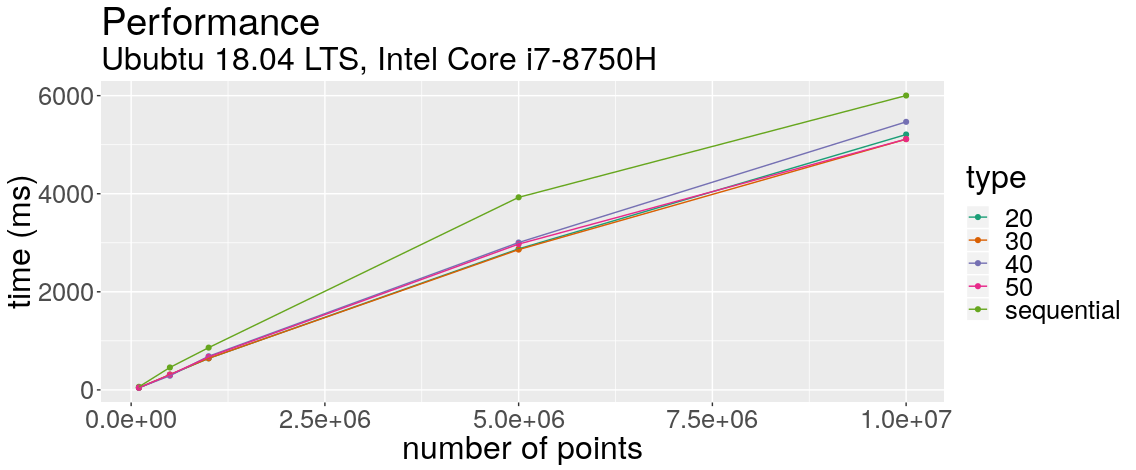
\includegraphics[width=1\textwidth, height=0.4\textheight]{performance}
		\caption{Performance data}
		\label{fig:performance}
	\end{figure}


\section{Conclusion}


	We`ve considered in details the process of designing and implementing the UAEM as well unified data structures for it. In this model a generic interface of a ``divide-and-conquer'' algorithm was created. This allows us to execute the algorithms which are implemented according to this model both sequentially and in parallel. Apart from that concatenable queue was implemented and served as the basis for the model described above.
	
	Using the data structure allowed to significantly reduce the time and computational resources for solving set of problems, such as constructing the convex hull. The algorithmic environment was implemented in Java programming language using its standard library. The main advantages of the developed algorithm are optimized preprocessing stage and the efficiently implemented merge step, due to the usage of concatenable queue.
	
	The performance comparison for both types of execution allows to conclude that the algorithm has high level of parallelism. We`ve achieved speedup of $28\%$ in the best case. It is easy to extend functionality of the created environment either by adding new or modifying existing algorithms. This flexibility is achieved by using the modular principle in its design and choosing optimal abstractions to represent algorithms.

\bibliography{article-SoCG-EA}
\end{document}
